\documentclass[a4paper,11pt, ctexart]{article}

\usepackage[english]{babel}

\usepackage[a4paper,top=4cm,bottom=4cm,left=4cm,right=4cm,marginparwidth=1.75cm]{geometry}

\usepackage{fontspec}
\usepackage{amsmath}
\usepackage{graphicx}
\usepackage[colorlinks=true, allcolors=blue]{hyperref}
\usepackage{xeCJK}
\usepackage{xcolor}
\usepackage{listings}

\definecolor{codegreen}{rgb}{0,0.6,0}
\definecolor{codegray}{rgb}{0.5,0.5,0.5}
\definecolor{codepurple}{rgb}{0.58,0,0.82}
\definecolor{backcolour}{rgb}{0.95,0.95,0.92}

\lstdefinestyle{mystyle}{
  backgroundcolor=\color{backcolour}, commentstyle=\color{codegreen},
  keywordstyle=\color{magenta},
  numberstyle=\tiny\color{codegray},
  stringstyle=\color{codepurple},
  basicstyle=\ttfamily\footnotesize,
  breakatwhitespace=false,         
  breaklines=true,                 
  captionpos=b,                    
  keepspaces=true,                 
  numbers=left,                    
  numbersep=5pt,                  
  showspaces=false,                
  showstringspaces=false,
  showtabs=false,                  
  tabsize=2
}

\lstset{style=mystyle}

\title{CP2024-II HW0105}
\author{Hsin-Jui Lin}

\begin{document}
\maketitle

\section{Taiko Music Generator (20 pts)}
\textbf
Have you ever heard of or played the game Taiko no Tatsujin(太鼓の達人)? Here is how to game play{\href{https://taiko.namco-ch.net/taiko/tc/howto/index.php}{\tiny link}}. It's a rhythm game where players hit taiko-notes by striking the center or rim of a taiko drum. You might have seen taiko arcade outside, such as the ones near our school in Gongguan. But did you know that this game is also available on various platforms like Nintendo, PS, mobile apps (RHYTHM CONNECT{\href{https://app-ttrc.taiko-ch.net/ch/}{\tiny link}}), and even on computers through simulators (Taiko-san Daijiro)? Notably, simulators allow users to play their own taiko music by creating custom chart(譜面) and music.

\begin{figure}[h]
    \centering
    
\includegraphics[width=0.8\textwidth]{assets/taiko-no-tatsujin.jpg}
    \caption{Taiko no Tatsujin game}
\end{figure}

In the simulator, the game is run by reading in .tja files, which are considered charts controlling the taiko-notes. However, the contents of tja files are not very intuitive. Therefore, this time, I want you to develop program which can convert tja files into a json file that represents the music and taiko-notes's timeline using timestamp notation. In other words, the goal is to map the taiko-notes to specific seconds on the music timeline.

\subsection{tja file}

(See this website{\href{https://home.gamer.com.tw/artwork.php?sn=5189897}{\tiny link}} and download sample{\href{https://drive.google.com/drive/folders/1vyX1WX_bAHkd51JxgZWU8D_5Nfe-DGVw?usp=share_link}{\tiny link}} tja file) To make it easier for you to analyze tja files, I also provide a simple explanation. This is the typical structure of a tja file:

\begin{lstlisting}
// ===================================================
//                  Header Area
//  Header area set the tja global and inital setting
// ===================================================
TITLE
.
.
.
// ===================================================

// ===================================================
//                  Body Area 1
//          Body area set the music chart value
// ===================================================
COURSE
// Music and Chart Setting in this course
.
#START
// Chart Contents
.
.
#END
// ===================================================

// ===================================================
//                  Body Area n
//        Body amount is be decide according to
//              how many course does it have 
//                Range from 1 ~ 5 totally
// ===================================================
COURSE
// Music and Chart Setting in this course
.
#START
// Chart Contents
.
.
#END
// ===================================================
\end{lstlisting}

You only need to get the values corresponding to the following key (ignore the others):

\begin{itemize}
\item 
{
    BPM:[float]
}
\item 
{
    OFFSET:[float]
}
\item 
{
    COURSE:[string|uint]  // Easy:0, Normal:1, Hard:2, Oni:3, Edit:4
}
\item 
{
    \#START
}
\item 
{
    \#MEASURE beat[uint]/note[uint]
}
\item 
{
    \#BPMCHANGE [float]
}
\item 
{
    \#END
}
\item 
{
    xxxxxxxxx, // chart content
}
\end{itemize}

\subsection{Output Timeline Chart json}
To output as a chart json, here is the following is the json format structure:

\begin{lstlisting}
{
  "data": [
        {
            "course": "taiko difficulty number [uint]",
            "chart": [
                ["taiko-note number [uint]", "timestamp [float]"], 
                                ...
            ]
        },
        {
            "course": ...
            "chart": [
                ...
            ]
        },
        ...
    ]
}
\end{lstlisting}


You just need to detect these taiko-notes (Figure 3):
\begin{itemize}
\item 
{
    DON(Red): 1 
}
\item 
{
    KA(Blue): 2
}
\item 
{
    BIGDON(Big Red): 3
}
\item 
{
    BIGKA(Big Blue): 4
}
\item 
{
    Blank(Nothing): 0 (5, 6, 7, 8, 9)
}

\end{itemize}

\begin{figure}[h]
    \centering
    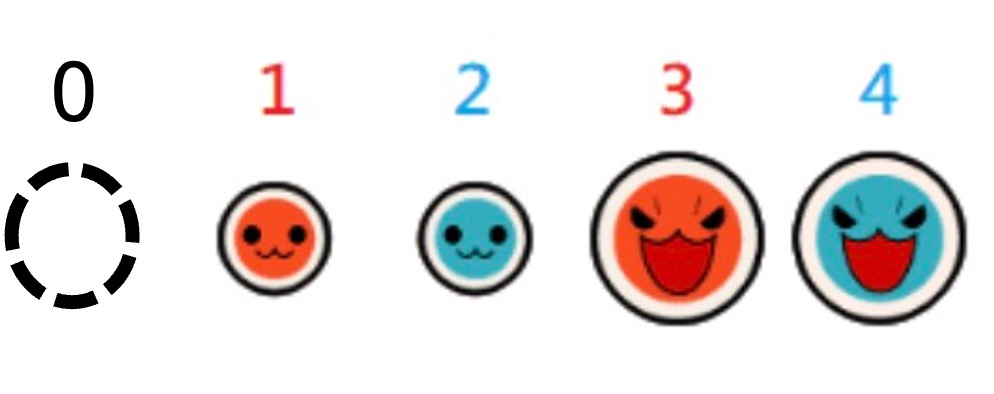
\includegraphics[width=0.6\textwidth]{assets/taiko-note.jpg}
    \caption{Taiko Notes}
\end{figure}

\subsection{Convert tja file into Timeline Chart}
After understanding which values to extract from the tja files and knowing their principles, in order to map taiko-notes to the music timeline, you need to understand a formula algorithm:

$$ duration = \frac{60}{bpm} * \frac{beat}{Length(chart)} * \frac{4}{note} $$

You must track the BPM, beat, and note value in the chart to determine the duration. There's tja file example:

\begin{lstlisting}
// 怪物.tja
BPM:170
OFFSET:-1.646
COURSE:Normal

#START
#MEASURE 4/4
1011, // duration = (60/170)*(4/4)*(4/4) ~= 0.352
\end{lstlisting}

Then it looks like Figure 4{\href{https://youtu.be/Fv2t7NqJVZE?si=UTd9gqh7ALQBbVu8&t=13}{\tiny link}}.

\begin{figure}[h]
    \centering
    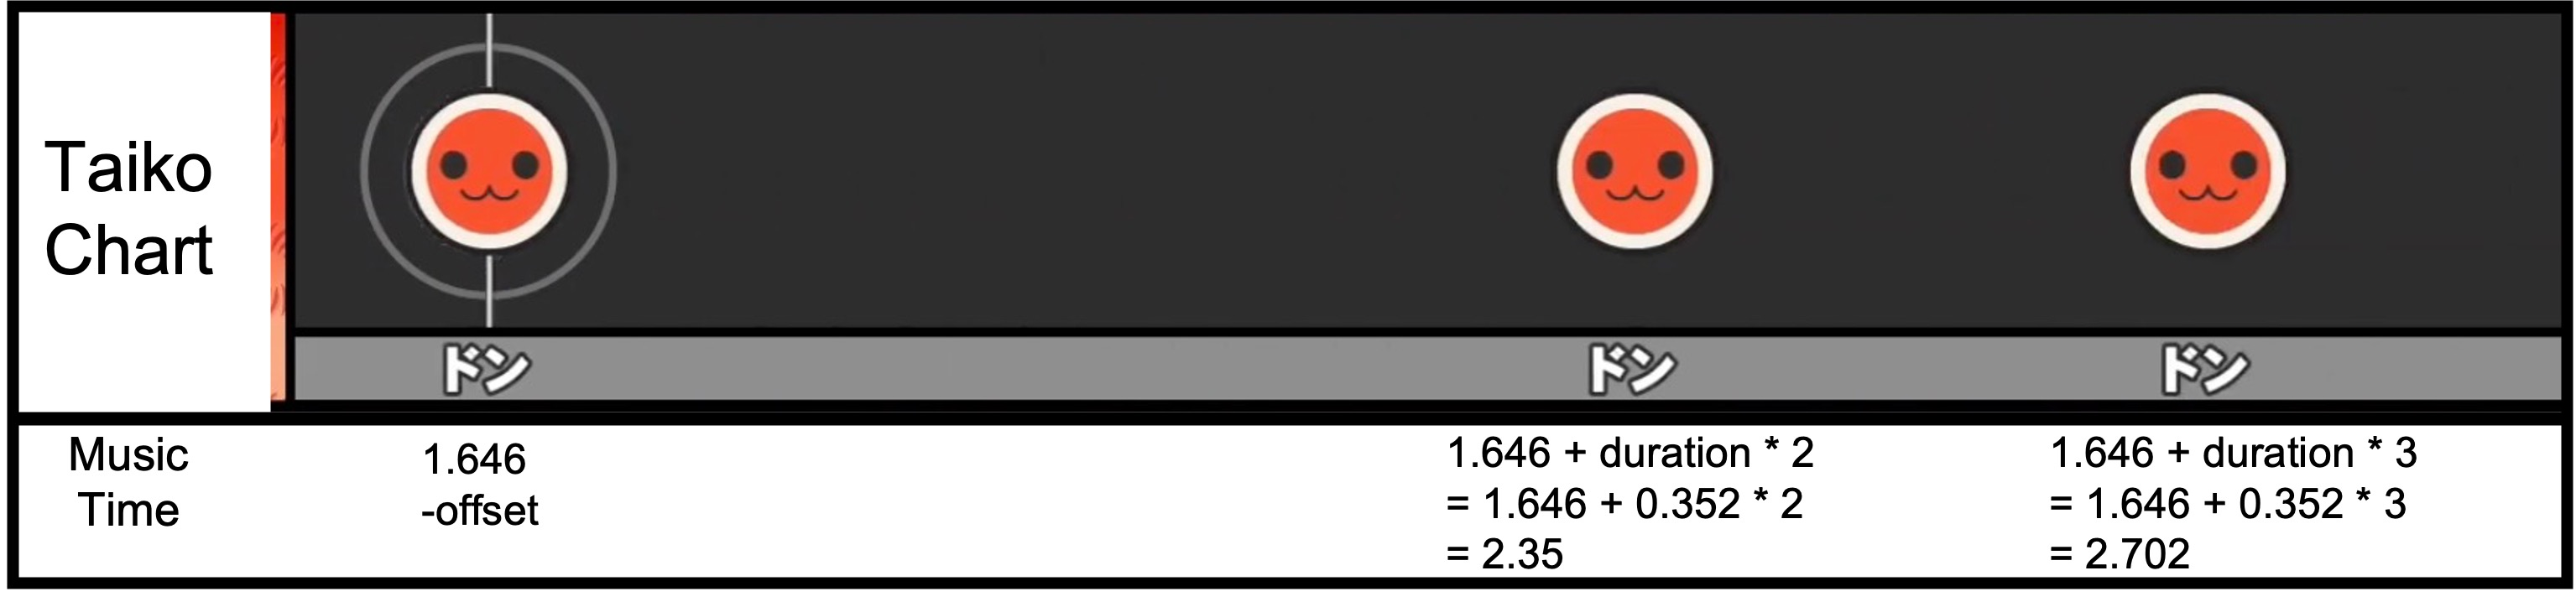
\includegraphics[width=0.8\textwidth]{assets/timeline-chart-example.jpg}
    \caption{Timeline Chart Example}
\end{figure}

And chart.json looks like:
\begin{lstlisting}
{
  "data": [
        {
            "course": 1,
            "chart": [
                [1, 1.646],
                [1, 2.35],
                [1, 2.702]
            ]
        }
    ]
}
\end{lstlisting}

Before calculating duration, beware that if $ Length(chart) < beat $, then you have to extend the length of chart content to $ lcm(Length(chart), beat) $. But if $Length(chart) = 0$,  extend 0's number of beat:

\begin{lstlisting}
#MEASURE 6/4
1, -> 100000, duration = 0.4
, -> 000000, duration = 0.4
02, -> 000200, duration = 0.4
102, -> 100020, duration = 0.4
2401, -> 200400000100, duration = 0.2
\end{lstlisting}

So if bpm = 150 and offset = 0 currently. And that is to be:
\begin{lstlisting}
"chart": [
    [1, 0],
    [2, 6],
    [1, 7.2],
    [2, 8.8],
    [2, 9.6],
    [4, 10.2],
    [1, 11.4]
]
\end{lstlisting}

\subsection{Generate Taiko Music}
You can go in this website{\href{https://huggingface.co/spaces/ryanlinjui/taiko-music-generator}{\tiny link}} website and generate taiko music by inputting the chart json file and the music ogg file. You can see the Figure 5 example.

\begin{figure}[h]
    \centering
    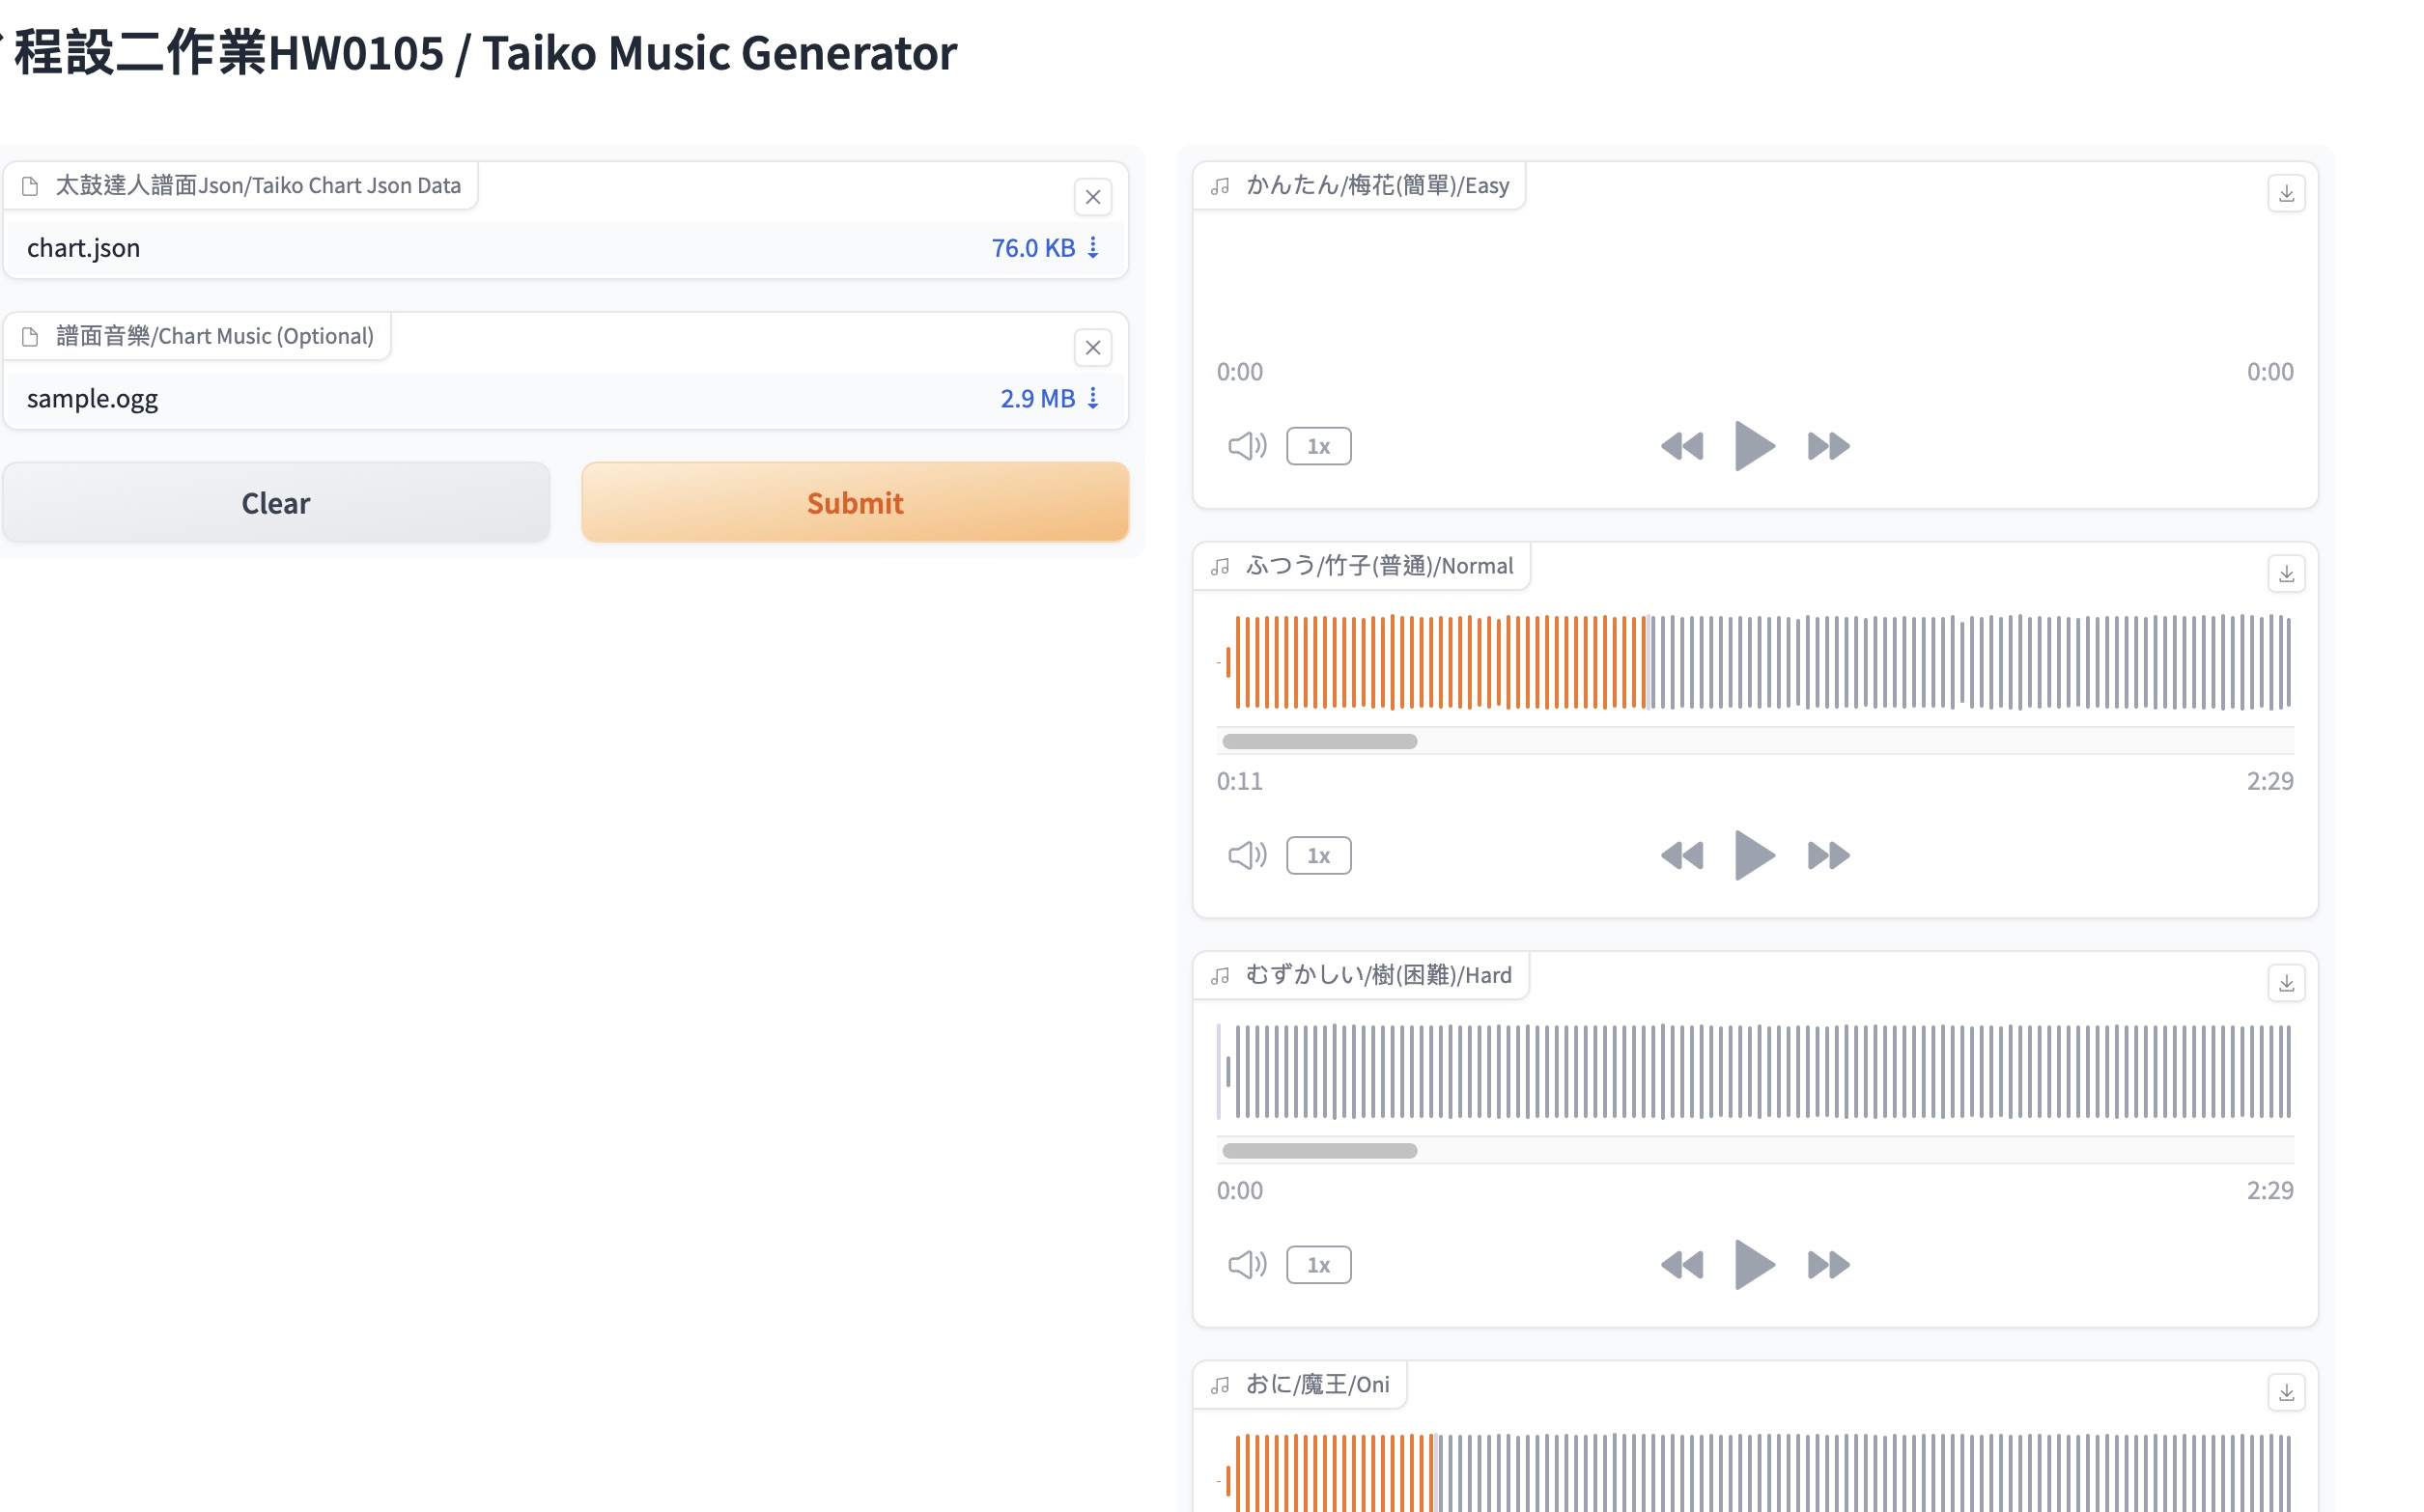
\includegraphics[width=0.8\textwidth]{assets/web.jpg}
    \caption{Taiko Music Generator Website}
\end{figure}

\subsection{Example by Running Program}
Again, the purpose of your program is to convert the contents of tja files into output the contents of chart json files. There's the input and output example following below:

\subsubsection{Input}
\begin{lstlisting}
TITLE:
SUBTITLE:
BPM:170
WAVE:
OFFSET:-1.646
DEMOSTART:35.15
SONGVOL:100
SEVOL:100


COURSE:Oni
LEVEL:7
BALLOON:2
SCOREINIT:
SCOREDIFF:
#START
11211122,
,
#END


COURSE:Hard
LEVEL:6
BALLOON:2,24
SCOREINIT:
SCOREDIFF:
#START
10101212,
#END

COURSE:Normal
LEVEL:5
BALLOON:14,7,18,7
SCOREINIT:930,4870
SCOREDIFF:305

#START
1011,
10010101,
,
#END


COURSE:Easy
LEVEL:3
BALLOON:11,5,14,5
SCOREINIT:
SCOREDIFF:
#START
1,
1,
1,
12,
,
#END
\end{lstlisting}

\subsubsection{Output}
\begin{lstlisting}
{
	"data": [
		{
			"course": 3,
			"chart": [
				[1, 1.646000],
				[1, 1.822471],
				[2, 1.998941],
				[1, 2.175412],
				[1, 2.351882],
				[1, 2.528353],
				[2, 2.704823],
				[2, 2.881294]
			]
		},
		{
			"course": 2,
			"chart": [
				[1, 1.646000],
				[1, 1.998941],
				[1, 2.351882],
				[2, 2.528353],
				[1, 2.704823],
				[2, 2.881294]
			]
		},
		{
			"course": 1,
			"chart": [
				[1, 1.646000],
				[1, 2.351882],
				[1, 2.704824],
				[1, 3.057765],
				[1, 3.587177],
				[1, 3.940118],
				[1, 4.293059]
			]
		},
		{
			"course": 0,
			"chart": [
				[1, 1.646000],
				[1, 3.057765],
				[1, 4.469530],
				[1, 5.881294],
				[2, 6.587176]
			]
		}
	]
}
\end{lstlisting}

If there is an error issue occurred, you have to output nothing and exit the program.

For your convenience, I'll provide some files{\href{https://drive.google.com/drive/folders/1421NayATBfN9E9qMTdI7dUAwQZCzdoyv?usp=sharing}{\tiny link}} for your development and testing:
\begin{itemize}
\item 
{
    taiko.h (optional to use)
}
\item 
{
    sample tja and ogg files
}
\item 
{
    sample chart json files
}
\item 
{
    urls of people playing Taiko no Tatsujin on YouTube (for validating the taiko music that you generate)
}
\end{itemize}

\end{document}